\documentclass[a4paper]{article}

%Пакеты для математических символов:

\usepackage{amsmath} % американское математическое сообщество.
\usepackage{amssymb} % миллион разных значков и готический, ажурный шрифты.
\usepackage{amscd} % диаграммы, графики.
\usepackage{amsthm} % окружения теорем, определений и тд.
\usepackage{physics} % основные физические символы
\usepackage{tikz-feynhand} % Ферми диограммы
%\usepackage{latexsym} % треугольники и пьяная стрелка.

%пакеты для шрифтов:
%\usepackage{euscript} % прописной шрифт с завитушками.
\usepackage{MnSymbol} % Значеки доказательства
\usepackage{verbatim} % улучшенный шрифт "пишущей машинки".
\usepackage{array} % более удобные таблицы.
%\usepackage{multirow} % мультистолбцы в таблицах.
%\usepackage{longtable} % таблицы на несколько страниц.
%\usepackage{latexsym}
\usepackage{collectbox} % Добавляет коробочки, можно складывать туда текст)

\usepackage[backend=biber, style=gost-numeric]{biblatex} % Литература по госту

    
%Пакеты для оформления:
\RequirePackage[center, medium]{titlesec}% Стиль секций и заголовков
%\usepackage[x11names]{xcolor} % 317 новых цветов для текста.
\usepackage{float} % Позволяет использовать H, h! для локации фигур
%\usepackage{multicol} % набор текста в несколько колонн.
\usepackage{graphicx} % расширенные возможности вставки стандартных картинок.
\usepackage{subcaption} % возможность вставлять картинки в строчку
%\usepackage{caption} % возможность подавить нумерацию у caption.
\usepackage{wrapfig} % вставка картинок и таблиц, обтекаемых текстом.
\usepackage{cancel} % значки для сокращения дробей, упрощения, стремления.
\usepackage{misccorr} % в заголовках появляется точка, но при ссылке на них ее нет.
\usepackage{indentfirst} % отступ у первой строки раздела
%\usepackage{showkeys} % показывает label формул над их номером.
%\usepackage{fancyhdr} % удобное создание верхних и нижних колонтитулов.
%\usepackage{titlesec} % еще одно создание верхних и нижних колонтитулов
\usepackage{hyperref} % Ссылки как внешние так и внутренние
\hypersetup{
    colorlinks=true,
    linkcolor=black,
    filecolor=magenta,      
    urlcolor=cyan,
    pdftitle={Overleaf Example},
    pdfpagemode=FullScreen,
    }

    
\usepackage{xcolor} %Позволяет перекрасить все страници
\definecolor{mycolor}{RGB}{244,228,215} %Цвет перекраски


%Пакеты шрифтов, кодировок. НЕ МЕНЯТЬ РАСПОЛОЖЕНИЕ.
\usepackage[utf8]{inputenc} % кодировка символов.
%\usepackage{mathtext} % позволяет использовать русские буквы в формулах. НЕСОВМЕСТИМО С tempora.
\usepackage[T1, T2A]{fontenc} % кодировка шрифта.
\usepackage[english, russian]{babel} % доступные языки.

%tikz:
\usepackage{tikz} % tikz
\usetikzlibrary{decorations.text} % позволяет делать текст вдоль кривой.
\usetikzlibrary{external} % позволяет кэшировать рисунки tikz.


\usepackage{pgfplotstable}

%Отступы и поля:
%размеры страницы А4 11.7x8.3in
\textwidth=7.3in % ширина текста
\textheight=10in % высота текста
\oddsidemargin=-0.5in % левый отступ(базовый 1дюйм + значение)
\topmargin=-0.5in % отступ сверху до колонтитула(базовый 1дюйм + значение)


%Сокращения
%Скобочки
\newcommand{\inrad}[1]{\left( #1 \right)}
\newcommand{\inner}[1]{\left( #1 \right)}
\newcommand{\infig}[1]{\left\{ #1 \right\}}
\newcommand{\insqr}[1]{\left[ #1 \right]}
\newcommand{\ave}[1]{\left\langle #1 \right\rangle}

%% Красивые <= и >=
\renewcommand{\geq}{\geqslant}
\renewcommand{\leq}{\leqslant}

%%Значек выполнятся
\newcommand{\per}{\hookrightarrow}

%%Векторная алгебра
\newcommand{\rot}{\text{rot}}
\renewcommand{\div}{\text{div}}
\renewcommand{\grad}{\text{grad}}

%% Более привычные греческие буквы
\renewcommand{\phi}{\varphi}
\renewcommand{\epsilon}{\varepsilon}
\newcommand{\eps}{\varepsilon}
\newcommand{\com}{\mathbb{C}}
\newcommand{\re}{\mathbb{R}}
\newcommand{\nat}{\mathbb{N}}
\newcommand{\stp}{$\filledmedtriangleleft$}
\newcommand{\enp}{$\filledmedsquare$}

%%Тензорный анализ ОТО теория поля
\newcommand{\Li}[1]{\mathfrak{L}_{#1}}
\newcommand{\crist}[3]{\cfrac{1}{2} \inner{g_{#1#2,#3} + g_{#1#3,#2} - g_{#2#3,#1}}}
\newcommand{\piv}[2]{\cfrac{\partial #1}{\partial #2}}


\newcommand{\redd}[1]{\textcolor{red}{#1}}%Красный текст
\newcommand{\newdot}{\textbullet \hspace{0.5em}}%абзац начинающийся с точки


\makeatletter
\newcommand{\sqbox}{%
    \collectbox{%
        \@tempdima=\dimexpr\width-\totalheight\relax
        \ifdim\@tempdima<\z@
            \fbox{\hbox{\hspace{-.5\@tempdima}\BOXCONTENT\hspace{-.5\@tempdima}}}%
        \else
            \ht\collectedbox=\dimexpr\ht\collectedbox+.5\@tempdima\relax
            \dp\collectedbox=\dimexpr\dp\collectedbox+.5\@tempdima\relax
            \fbox{\BOXCONTENT}%
        \fi
    }%
}
\makeatother
\newcommand{\mergelines}[2]{
\begin{tabular}{llp{.5\textwidth}}
#1 \\ #2
\end{tabular}
}
\newcommand\tab[1][0.51cm]{\hspace*{#1}}
\newcommand\difh[2]{\frac{\partial #1}{\partial #2}}

\newcounter{customsection}
\newcommand{\mysection}[1]{
    \refstepcounter{customsection}
    \addcontentsline{toc}{section}{Appendix \arabic{customsection}: #1} % Добавляет запись в содержание
    \noindent\textbf{Appendix \arabic{customsection}: #1} % Как выглядит в тексте 
} % Независимые секции (аппендиксы) 



\numberwithin{equation}{section}


\begin{document}

\newpage
\tableofcontents
\newpagestyle{main}{
\setfootrule{0.4pt}
\setfoot{}{\thepage}{\sectiontitle }}
\pagestyle{main}


\section{Введение}

\subsection{Мотивация}

Предпосылки открытия очарованного бариона $\Lambda_c$ появились в 1975 году, когда в результате наблюдения аномалии в распаде $e^+ e^- \to e^+ + \mu^- + E_{miss}$ (см. \textbf{\cite{PhysRevLett1975}}) было высказано предположение о существовании заряженного лёгкого очарованного бариона. Открытие на достаточном уровне значимости произошло более чем 10 лет спустя на коллайдере SPEAR (см. \textbf{\cite{Avery1988}}) по распаду $\Lambda_c \to p K^- \pi^+$. 

$\Lambda_c$, будучи самым лёгким из очарованных барионов, распадается исключительно посредством слабого взаимодействия, что позволяет изолировать и исследовать вклад этого взаимодействия в барионных системах.
В частности, канал $\Lambda_c \rightarrow \Lambda l \nu_l$, где $l = e, \mu$, а распад с продуктом $l = \tau$ подавлен в силу закона сохранения 4-импульса:

\begin{equation*}
    m_{\Lambda_c} = 2.28646\,\text{GeV} < 2.89261\,\text{GeV} = 1.77693\,\text{GeV} + 1.11568\,\text{GeV} = m_{\tau} + m_{\Lambda}.
\end{equation*}

Бранчинговые отношения для полулептонных распадов $\Lambda_c \rightarrow \Lambda l \nu_l$, где $l = e, \mu$, были измерены в нескольких работах. Для канала $\Lambda_c \rightarrow \Lambda e \nu_e$ измеренное бранчинговое отношение составляет $B(\Lambda_c \rightarrow \Lambda e \nu_e) = 3.56 \pm 0.13\%$, как указано в статье \cite{CLEO2023}. Для канала $\Lambda_c \rightarrow \Lambda \mu \nu_{\mu}$ измеренное бранчинговое отношение равно $B(\Lambda_c \rightarrow \Lambda \mu \nu_{\mu}) = 3.48 \pm 0.17\%$ согласно \cite{CLEO2023}.

Полулептонные распады $\Lambda_c$ являются удобным и относительно простым случаем для исследования переходов тяжелого кварка в лёгкий, что позволяет точнее проверять предсказания теоретических моделей, таких как эффективная теория тяжёлых кварков (HQET) и квантовая хромодинамика на решётке (LQCD). Проверка этих моделей с помощью экспериментов может не только подтвердить их верность, но и выявить отклонения от стандартной модели, что потенциально указывает на существование новой физики, включая новые взаимодействия или экзотические частицы.

\subsection{Отличие от работы CLEO}

Измерение форм-фактора $\Lambda_c \rightarrow \Lambda l \nu_l$ важно для проверки результатов предыдущего эксперимента \textbf{\cite{CLEO2023}}, в котором был измерен форм-фактор $\Lambda_c \rightarrow \Lambda e \nu_e$. Важно сравнить методологические и экспериментальные аспекты текущего исследования с работой команды CLEO.

Прежде всего, команда CLEO сделала предположение о том, что спин бариона $\Lambda$ равномерно распределён. Это предположение оказывает влияние на значение спиральности, которое напрямую входит в уравнение для форм-фактора. В данной работе предлагается более точное измерение распределения направлений спина, основанное на анализе распада в канале $\Lambda_c^+ \rightarrow \Lambda \pi^+$. Этот подход позволяет уменьшить систематические ошибки и повысить точность вычислений.

Второе важное отличие заключается в использовании независимого источника данных. В то время как команда CLEO использовала данные, собранные с детектора "CLEO" на Корнельском электронном накопительном кольце (Cornell Electron Storage Ring), в настоящей работе анализ проводился на детекторе "Belle", установленном на ускорителе "KEK". Это не только обеспечивает независимую проверку результатов, но и позволяет уточнить их с учётом различий в экспериментальных установках.

Наконец, команда CLEO не проводила анализа полулептонного распада $\Lambda_c \rightarrow \Lambda \mu \nu_\mu$, что является существенным упущением. В данном исследовании этот канал был тщательно изучен, что позволяет расширить понимание полулептонных распадов и улучшить тесты на универсальность лептонов.

Таким образом, данная работа вносит вклад в дальнейшее изучение свойств бариона $\Lambda_c$ и уточнение результатов, полученных в предыдущих исследованиях.

\subsection{Модели и теоретические предсказания}

Как уже было сказано выше, на данный момент существуют численные методы вычисления форм-факторов, основанные на различных приближениях или моделях. Все они дают различные результаты (см. таблицу \ref{tb:chd}). Поскольку сильное взаимодействие сложно поддаётся теоретическим расчётам из-за отсутствия малого параметра, результаты могут быть проверены только экспериментально.

\begin{table}[H]
    \centering
    \caption{Форм-факторы полулептонных распадов $\Lambda_c \to \Lambda$ для $q^2 = 0$.}
    \begin{tabular}{|c|c|c|c|c|c|c|}
    \hline
    Form Factor & $\mathfrak{F}_1^V(0)$ & $\mathfrak{F}_2^V(0)$ & $\mathfrak{F}_3^V(0)$ & $\mathfrak{F}_1^A(0)$ & $\mathfrak{F}_2^A(0)$ & $\mathfrak{F}_3^A(0)$ \\
    \hline
    \textbf{\cite{QCD2021}} & 0.687(138) & 0.486(117) & 0.164(80) & 0.539(101) & -0.388(100) & -0.359(283) \\
    \hline
    \textbf{\cite{BagModel1989}} & 0.35 & 0.09 & 0.25 & 0.61 & -0.04 & -0.11 \\
    \hline
    \textbf{\cite{RQM2016}} & 1.14 & 0.072 & 0.252 & 0.517 & -0.697 & -0.471 \\
    \hline
    \textbf{\cite{QSR2009}} & 0.665 & 0.285 & --- & 0.665 & -0.285 & --- \\
    \hline
    \textbf{\cite{LFCQM2018}} & 0.468 & 0.222 & --- & 0.407 & -0.035 & --- \\
    \hline
    \end{tabular}
    \label{tb:chd}
\end{table}


\section{Экспериментальная установка}

\subsection{Коллайдер KEK}
Ускоритель KEKB является электрон-позитронным коллайдером, состоящим из двух 
колец, пересекающихся в одной точке под углом $22\,\text{mrad}$, что позволяет измерять CP-асимметрию. 
Пучки электронов и позитронов сталкиваются с энергией $8\,\text{GeV}$ и $3.5\,\text{GeV}$ соответственно.
Пучки рождаются на фотонной фабрике и, проходя через линейный ускоритель, где разгоняются до скорости, близкой к скорости света, 
передаются в основные кольца. В режиме накопления пучка подача происходит непрерывно, а в нормальном режиме 
сбора данных - периодически, раз в несколько миллисекунд.

Основной целью было производство большого количества B-мезонов. Работа ускорителя началась в декабре
1998 года и закончилась в конце июня 2010 года. За это время KEKB установил мировой
рекорд по светимости - $2.11\times 10^{34} cm^{-2}s^{-1}$, который на сегодняшний день был
превзойдён только на коллайдере SuperKEKB - усовершенствованной версии, собранной
на основе KEKB. За все время было собрано $825.547fb^{-1}$.

\begin{figure}[H]
    \centering
    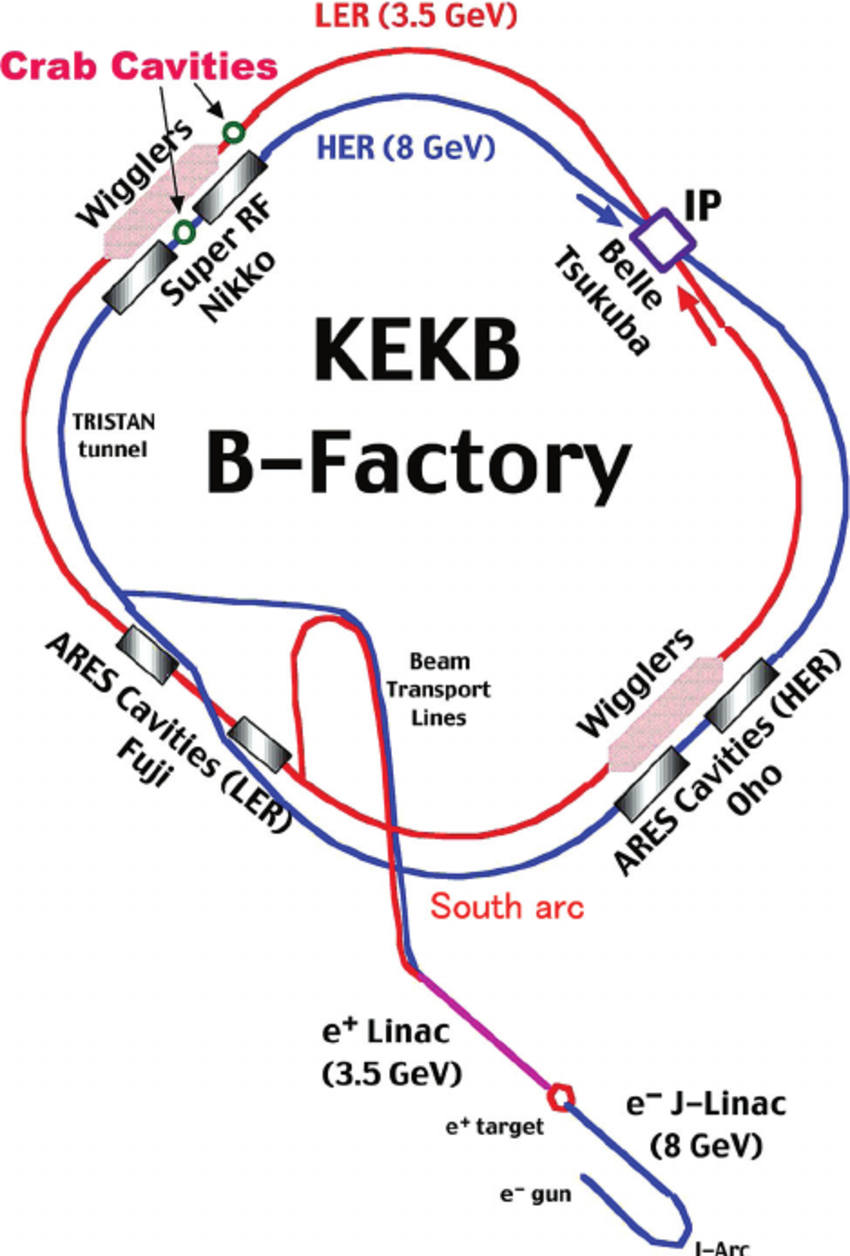
\includegraphics[width=0.5\linewidth]{img/kekb.png}
    \caption{Ускорительный комплекс KEKB}
    \label{the:kek}
\end{figure}

\subsection{Детектор Belle}

Детектор Belle охватывал весь азимутальный угол, а также перекрывал 
часть полярного угла от $17^{\circ} $ до $150^{\circ} $, что соответствует $0.74$
полного телесного угла. Установка окружала точку взаимодействия и состояла 
из вершинного кремниевого детектора (SVD), центральной дрейфовой 
камеры (CDC) из 50 цилиндрических слоёв, массива аэрогелевых черенковских 
счётчиков (ACC), системы измерения времени пролёта (TOF) из сцинтилляционных 
счётчиков, электромагнитного калориметра (ECL), изготовленного из кристалов 
йодида цезия (CsI), и переднего калориметра (EFC), расположенных внутри 
сверхпроводящего соленоида, обеспечивающего магнитное поле величиной 
$1.5 Tl$. В железном ярме электромагнита был расположен детектор $K_L^0$ мезонов 
и $\mu$ (KLM), составленный из стеклянных резистивных плоских камер. 
Общий вид детектора Belle показан на рис. \ref{the:belle}. Подробно о поддетекорах 
и востановлении события в \redd{ссылка на аппендикс}.

\begin{figure}[H]
    \centering
    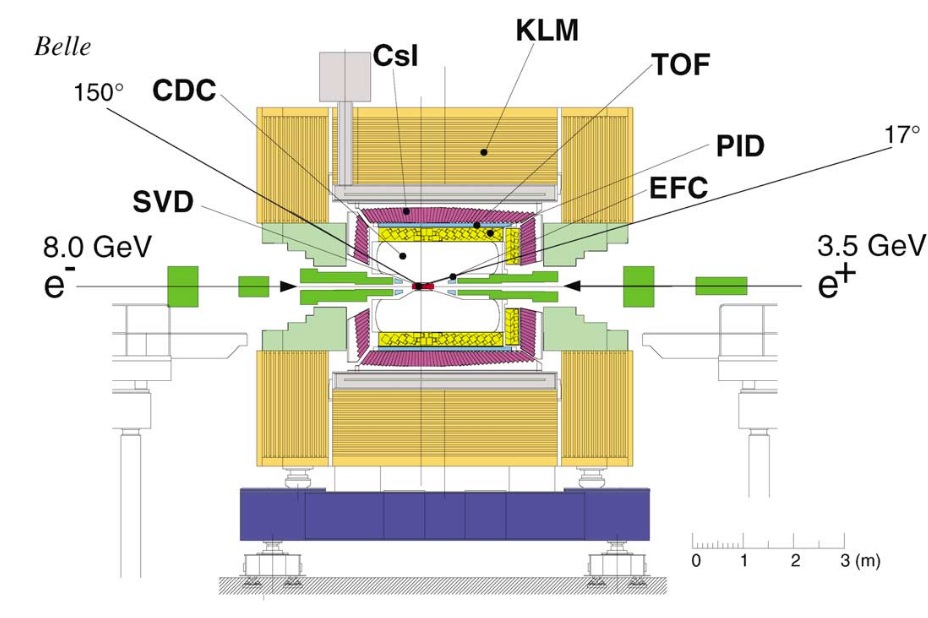
\includegraphics[width=0.8\linewidth]{img/the_belle.png}
    \caption{Декткор Belle в сечении}
    \label{the:belle}
\end{figure}





\section{Каналов тагирования}
\label{taging}
\subsection{Тагирование $\Lambda_c$}

Для восстановления распадов $\Lambda_c$-барионов и определения импульса недетектируемого нейтрино применяется тагирование по заряду, аромату и барионному числу. Будем предполагать, что $\Lambda_c$ образуется из $\bar{c}$-кварка и подхваченных из вакуума недостающих кварков. В таком случае будем называть систему центромасс $c$-кварка $X_c$, то есть неизвестная очарованная частица, которая фактически может быть не одной, а несколькими частицами сразу.

\begin{figure}[h!]
    \centering
    \begin{tikzpicture}
        \begin{feynhand}
            \vertex [particle] (e) at (-2,1) {$e^-$};
            \vertex [particle] (ae) at (-2,-1) {$e^+$};
            
            \vertex [particle] (photon) at (0,0);
            \vertex (w1) at (1, 0);
            
            \vertex [particle] (c) at (3,1) {$c$};
            \vertex [particle] (anti_c) at (3,-1) {$\bar{c}$};
        
            \propag [fermion] (e) to (photon);
            \propag [anti fermion] (ae) to (photon);
            \propag [photon] (photon) to  [edge label=$\gamma*$]  (w1);
            \propag [fermion] (w1) to (c);
            \propag [anti fermion] (w1) to (anti_c);
        \end{feynhand}
    \end{tikzpicture}
\end{figure}

Для того чтобы определить состав $X_c$, необходимо, чтобы соблюдались законы 
сохранения барионного числа, аромата, заряда, а также 4-импульса. Такая 
технология называется тагированием \textcolor{red}{ссылка на работу}. В 
результате получим, что в $X_c$ будет входить хотя бы один барион и кварки 
$u c d$, а также любые пары $q \bar{q}$. В итоге возможны следующие варианты 
$X_c$. Также важно понимать, что чем больше частиц содержит $X_c$, тем менее 
вероятно событие с такой комбинацией, так как новые частицы требуют 
дополнительных кварковых пар, создание которых требует больше энергии. 
Кроме того, при добавлении новых частиц время работы программы увеличивается 
экспоненциально, так как сложность алгоритма $\mathcal{O}(\prod_n N_n)$ 
(где $N_n$ количестов задетектированных частиц типа $n$ в событии).

В работе рассматриваются $X_c \to \Lambda^{tag}_c; \Lambda^{tag}_c \pi^- \pi^-; \Lambda^{tag}_c \pi^+ \pi^- \pi^+ \pi^-; D^0 p; D^+ p \pi^-; D*^0 p; D*^+ p \pi^- $, 
чтобы отличать $\Lambda_c$ котрую тагируемую от тагирующей (той что является продуктом $X_c$), вторую обозначаим как $\Lambda^{tag}_c$.
Каналы распада прочих частиц будем импользовать заведомо изветные самые эффективные каналы, согласно \cite{PDGTablesBar} для барионов и \cite{PDGTablesMes} для мезонов.
\begin{figure}[h]
    \centering
    \begin{tabular}{c|c}
        Particle & Channels \\ \hline
        $D^0$ & $K^- \pi^+; K^- \pi^+ \pi^+ \pi^-; K^- K^+; K^0_s \pi^+ \pi^+; K^0_s \pi^0; K^+ K^- K_s^0$ \\
        $D^+$ & $K^- \pi^+ \pi^+; K^0_s; K^0_s \pi^+ \pi^+ \pi^-; K^+ K^- \pi^+$ \\
        $\Lambda^{tag}_c$ & $pK^-\pi^+; \Lambda^0 \pi^+; \Lambda^0 \pi^+ \pi^0; p K_s^0 \pi^0$ \\
        $D*^+$ & $D^0 \pi^0; D^0 \gamma$ \\
        $D*^+$ & $D^+ \pi^0; D^0 \pi^+$ \\
        $\pi^0$ & $\gamma \gamma$ \\
        $K_s^0$ & $\pi^+ \pi^-$
    \end{tabular}
    \label{fig:part_channels}
\end{figure}

\subsection{Критерии отбора}

В данном разделе изложены критерии отбора, принятые на основании работы \cite*{BelleDetector2002} и описанном в \ref{mes_mthods}. 
Имея на набор треков и их параметров, надо их классифицировать по типу частици оставившей этот трек. 

\newdot Фотоны классифицированы, но используемые при реконструкции событий, наложим дополнительное ограничение $E_\gamma > 50 \text{ MeV}$, поскольку фотоны с меньшей энергией трудно отличимы тормозных или индуцированных в сичтеме токов, 
что может привести к ошибочной интерпретации их как сигнальных фотонов.

\newdot Идентификация частиц по (PID):

Как уже известно для треков формируется значение правдоподобия $L(p,a)$ 
и в поледствии PID значение $\mathfrak{L}_{p_1/p_2}(a)$, поэтому на треки котрые хотим 
идентифицировать как частицу $p$ наложим следующие ограничения:

\begin{figure}[h]
    \centering
    \begin{tabular}{c|c}
        Гипотеза & Критекрий \\ \hline
        $p \& \bar p$ & $\mathfrak{L}_{p/K} < 0.6; \mathfrak{L}_{p/\pi} > 0.6$ \\
        $K^\pm$   & $\mathfrak{L}_{p/K} < 0.4; \mathfrak{L}_{K/\pi} > 0.6$ \\
        $\pi^{\pm}$ & все заряженные треки, не прошедшие идентификацию по вышеуказанным критериям \\
    \end{tabular}
\end{figure}

\newdot $K_s^0$-мезоны реконструируются по распаду $K_s^0 \to \pi^+ \pi^-$ из кандидатов, отобранных с помощью стандартного инструмента V0finder и собранных в таблице MdstVee2. Критерии отбора следующие:

$$
\left| M_{K_s^0} - M^{real}_{K_s^0} \right| < 30 \text{ MeV}; \ \rho_{K_s^0} > 1 \text{ мм}; \ z_{K_s^0} > 1 \text{ см}; \ \cos \theta_{K_s^0} > 0.99
$$

где $M^{real}_{K_s^0} = 497.611 \text{ MeV}$, $M_{K_s^0}$ — инвариантная масса пионов ($\pi^+ \pi^-$), собранных в $K_s^0$-мезон, $z_{K_s^0}$ и $\rho_{K_s^0}$ — цилиндрические координаты реконструированной вершины распада $K_s^0$-мезона в лабораторной системе отсчёта, а $\cos \theta_{K_s^0}$ — азимутальный угол между импульсом $K_s^0$ и направлением на его вершину распада.

\newdot $\pi^0$ -мезоны восстанавливались в распаде на два фотона, которые в
свою очередь реконструировались по кластерам энерговыделения в ECL.
Критерии отбора:
$$
\abs{M_{\pi^0} - M_{\pi^0}^{real}} < 15 MeV 
$$
После отбора стандартно были установлены погрешности для импульсов фотонов и выполнены фиты в вершину и массу.

\newdot Отбор $D$ -мезонов:

\begin{figure}[h]
    \centering
    \begin{tabular}{c|c}
        $D^0$ & $\abs{M_{D^0} - M^{real}_{D^0}} < 15 MeV$ \\
        $D^\pm$ & $\abs{M_{D^\pm} - M^{real}_{D^\pm}} < 15 MeV$ \\
        $D*^{\pm}$ & $\abs{M_{D*^\pm} - M^{real}_{D*^\pm}} < 3 MeV$ \\
        $D*^0$ & $\abs{M_{D*^0} - M^{real}_{D*^0}} < 3 MeV$ \\
    \end{tabular}
\end{figure}

Где $M^{real}_{D^\pm} = 1864.83 MeV; M^{real}_{D^0} = 1869.65 MeV; 
M^{real}_{D*^\pm} = 2010.26;  M^{real}_{D*^0} = 2006.85 MeV$. 
Так де на $D*$-мезоны накладываем ограничение:

\begin{equation}
        \abs{M_{D*} - M^d_{D}} < 15 MeV
\end{equation}

Где $ M^d_{D}$ --- масса $D$-мезона используемого для кобинации соответствующего. 
$D^*$. Так как ошибка собранного $D*$ мезона карелирует с собранным 
предврительно $D$-мезоном.



\section{Поиск $\Lambda_c$}

На основе выбранных нами каналов $X_c$ писанных в предыдущем разделе 
обираем события в котрых выполняется условие 

\begin{equation}
    \abs{p_{e^+} + p_{e^-} - p_{X_c}}^2 \leq 3 GeV
\end{equation}

Так как в идельных условиях эта влечина должна быть равна квадрату $M^{real}_{\Lambda_c} = 2226.46 MeV$, 
таким образом мы откинем множетво событий котрые затагировали 
возбужденные состояния $\Lambda_c$ или поряли трек.

В отобранных событиях мы будем собирать $\Lambda_c$ барионы. 
По каналам $\Lambda_c^+ \to \Lambda \pi^+; \Lambda \nu_e e^+; \Lambda \nu_\mu \mu^+$.



\newdot Для отбора $\Lambda \to p \pi$ требуем 

$$
\abs{ M_{\Lambda_c} - M^{real}_{\Lambda_c} } < 30 \text{ MeV}; 
\ \rho_{\Lambda_c} > 1 \text{ mm}; \ z_{\Lambda_c} > 1 \text{ cm}; 
\ \cos \theta_{\Lambda_c} > 0.99;
\ \mathfrak{L}_{p/K } > 0.6 
$$

\newdot Для отбора $e^\pm$ требем $p_{e^\pm} \geq 0.6 GeV$, чтобы долетел до SVD 
детектора где он в ходе $e^- \to \gamma e^- \to 2e^- e^+$ распадается электронн-фотонным ливнем, 
что позволяет его олично индетефицировать, поэтому критерий на $L(e) > 0.1$ не такой строгий.

\newdot Аналогично отбора $\mu^\pm$ требем $p_{\mu^\pm} \geq 0.6 GeV$, чтобы долетел до KLM, 
где идентификация мюнов еще лучше поэтому требуем $L(\mu) > 0.01$ 


\newdot Комбинируем $\Lambda_c$ с массовым окном $50 MeV$.

\newdot Независимо от работы \cite{BelleDetector2002}, среди моножетва $\infig{d_n}$, 
идентифицированных как кандидаты на дочерние продукты распада $\xi$ частици, 
можно использовать знание о том, что импульсы продуктов распада должны исходить 
из вершины распада. Это позволяет откорректировать измеренные импульсы с учётом 
погрешностей, чтобы они соответствовали данной гипотезе (в дальнейшем это будет 
называться "фит в вершину"). Аналогично, на основании инвариантной массы, 
известной для $\xi$, можно корректировать величины импульсов дочерних частиц 
так, чтобы $M_{p} = \sqrt{\sum_n \inner{p_n}_\gamma \inner{p_n}^\gamma}$ 
совпадала с $M^{real}_{\xi}$, где $p_n$ --- 4-импульс сответствующий $d_n$ 
из $\infig{d_n}$. Этот метод будет называться "фит в массу". Были использованы 
алгоритмы для фита в вершину и в массу принятые в коллаборации KEK, и описанные 
в \cite{Krohn2021}.

По итогу делаем фиты в вершину, а после в массу для всех собранных частиц это 
$\Lambda_c, D^{\pm}, D^0, D*^{\pm}, D*^0, \Lambda, K_s^0$.

\newdot Для импульс $X_c$ фитируем так чтобы $\abs{p_{e^+} + p_{e^-} - p_{X_c}}^2 = M^2_{\Lambda_c}$, 
подробно алгоритм описан в Appendix \ref{fit_rec_mass}. 

 









\mysection{Метод вычисления формфактора}

$\Lambda_c$ барион состит из $ucd$ кварков, в ходе распараспада 
$\Lambda_c \rightarrow \Lambda l \nu_l$ проискходит переход $c\to s$ 
посредством испускания $W^+$ бозона тоесть правиьно будет записвть $c\to s W^+$,
$W^+$ распадается на $W^+ \to l^+ \nu_l$, в итоге оставшиеся кварки 
$uds$ формируются в $\Lambda$ барион. Таким образом получим следующую 
феймановскую диаграмму.

\begin{figure}[H]
    \centering
    \begin{tikzpicture}
        \begin{feynhand}
            \vertex [particle] (i1) at (-3,4) {$u$};
            \vertex [particle] (i2) at (-3,3.5) {$d$};
            \vertex [particle] (i3) at (-3,3) {$c$};
            \vertex [particle] (f1) at (3,4) {$u$};
            \vertex [particle] (f2) at (3,3.5) {$d$};
            \vertex [particle] (f3) at (3,3) {$s$};
            \vertex (w1) at (0,3);
            \vertex (w2) at (0,2.5);
            \vertex (w3) at (0,2);
            \vertex (w4) at (1.5,1);
            \vertex [particle] (e) at (3,1.5) {$l^{-}$};
            \vertex [particle] (an) at (3,0.5) {$\bar{\nu}_{l}$};
            \propag [fermion] (i1) to (w1);
            \propag [fermion] (i2) to (w2);
            \propag [fermion] (i3) to (w3);
            \propag [fermion] (w1) to (f1);
            \propag [fermion] (w2) to (f2);
            \propag [fermion] (w3) to (f3);
            \propag [charged boson] (w3) to [edge label=$W^{-}$] (w4);
            \propag [fermion] (w4) to (e);
            \propag [anti fermion] (w4) to (an);        
        \end{feynhand}
    \end{tikzpicture}
\end{figure}

Переход $\Lambda_c \to \Lambda$ индуцирется слабым током $j_\mu$, 
котрый можно разложить по аксиальной и векторной части: 
$j_\mu = j_\mu^A + j_\mu^V$.
Обозначим волновые функции частиц
$B_{\Lambda_c} \inner{p_{\Lambda_c}, M_{\Lambda_c}} 
\to B_{\Lambda} \inner{p_{\Lambda}, M_{\Lambda}} 
+ l\inner{p_l, m_l} + \nu_l \inner{p_\nu, m = 0}$. 
Форм факторы выражаются как:
\begin{equation}
    \bra{B_{\Lambda_c} \inner{p_{\Lambda_c}, M_{\Lambda_c}}}
    j_\nu^V
    \ket{B_{\Lambda} \inner{p_{\Lambda}, M_{\Lambda}}} = 
    u_2^\dag \inner{\mathfrak F^V_1 \inner{q^2} \gamma_\nu + 
    \cfrac{\mathfrak F^V_2}{M_{\Lambda_c}} \inner{q^2} \sigma_{\mu\nu} q^\nu + 
    \cfrac{\mathfrak F^V_3}{M_{\Lambda_c}} \inner{q^2}q_\mu} u_1 
\end{equation}

\begin{equation}
    \bra{B_{\Lambda_c} \inner{p_{\Lambda_c}, M_{\Lambda_c}}}
    j_\nu^A
    \ket{B_{\Lambda} \inner{p_{\Lambda}, M_{\Lambda}}} = 
    u_2^\dag \inner{\mathfrak F^A_1 \inner{q^2} \gamma_\nu + 
    \cfrac{\mathfrak F^A_2}{M_{\Lambda_c}} \inner{q^2} \sigma_{\mu\nu} q^\nu + 
    \cfrac{\mathfrak F^V_3}{M_{\Lambda_c}} \inner{q^2}q_\mu} \gamma_5 u_1 
\end{equation}

Где $\gamma_\mu$ - матрци Диррака, $q_\mu$ - 4-импульс $W^+$ бозона,
$\sigma_{\mu\nu} = \cfrac{1}{2} \inner{\gamma_\mu \gamma_\nu - \gamma_\nu \gamma_\mu}$.

\redd{Дописать вывод связи форм фактора и спиральности}


\mysection{Алгоритм фита в массу потеряной частици}

\begin{figure}[h!]
    \centering
    \begin{tikzpicture}
        \begin{feynhand}
            \vertex [particle] (e) at (-3,0) {$e^-$};
            \vertex [particle] (ae) at (3,0) {$e^+$};
            
            \vertex [dot] (w1) at (0, 0) {};
                        
            \vertex [particle] (p1) at (1.964,-0.377) {$p_1$};
            \vertex [particle] (p2) at (-1.350,1.476) {$p_2$};
            \vertex [particle] (p3) at (1.582,1.222) {$p_3$};
            \vertex [particle] (lam_c) at (-1.667,-1.108) {$p_{taging}$};
        
            \propag [fermion] (e) to (w1);
            \propag [fermion] (ae) to (w1);
            \propag [fermion] (w1) to (p1);
            \propag [fermion] (w1) to (p2);
            \propag [fermion] (w1) to (p3);
            \propag [fermion] (w1) to (lam_c);
        \end{feynhand}
    \end{tikzpicture}
    \caption{Схема распада.}
    \label{fit_tag}
\end{figure}

Дано: $p_1, p_2, p_3$ --- это 4-импульсы продуктов распада (тагирующих выбранную частицу), представленных на рис.~\ref{fit_tag}. 
Также известны матрицы ковариаций компонент 3-импульса $\Xi_1, \Xi_2, \Xi_3$ для соответствующих частиц. 
$p_{\text{beam}}$ — это 4-импульс системы ($p_{\text{beam}}$), а $M_{\text{rec}}$ --- это масса недостающей (тагируемой) частицы.

Для поиска оптимального решения используется метод множителей Лагранжа. Поскольку мы минимизируем изменения импульсов с учётом их ошибок, применяем следующую функцию:

\begin{equation}
    \chi^2 = \sum_n \inner{p_{n}}_i  \inner{\Xi_n^{-1}}_{ij}  \inner{p_{n}}_j
\end{equation}

Функция Лагранжа с наложением ограничения имеет вид:

\begin{equation}
    M_{\text{rec}}^2 - (p_{\text{beam}} - \sum_n p_n)_\mu (p_{\text{beam}} - \sum_n p_n)^\mu = 0
\end{equation}

Полная функция Лагранжа с множителем Лагранжа $\lambda$ записывается следующим образом:

\begin{equation}
    \mathcal{L}(p_n, \lambda) = 
    sum_n \inner{p_{n}}_i  \inner{\Xi_n^{-1}}_{ij}  \inner{p_{n}}_j + 
    \lambda \left( M_{\text{rec}}^2 - (p_{\text{beam}} - \sum_n p_n)_\mu (p_{\text{beam}} - \sum_n p_n)^\mu \right)
\end{equation}

Для минимизации используется метод Ньютона-Рафсона. На каждом шаге вычисляются градиент (первая производная) и гессиан (матрица вторых производных) функции Лагранжа:

\begin{equation}
    \nabla \mathcal{L}(x_n) = c_n, \Delta \otimes \Delta \mathcal{L}(x_n)  = \hat{A}_n
\end{equation}

где $x_n$ — это вектор параметров на $n$-м шаге. Затем на каждом шаге решается система уравнений для обновления параметров:

\begin{equation}
    \hat{A}_n \, \delta x_{n+1} = -c_n
\end{equation}

После чего параметры обновляются:

\begin{equation}
    x_{n+1} = x_n + \delta x_{n+1}.
\end{equation}



\section{Литература}

\begin{thebibliography}{99}

    \bibitem{Avery1988} 
    Avery P., Blanco R., Liu K., et al. Observation of the Charmed Baryon $\Lambda^+_c$ at SPEAR // Phys. Rev. Lett. 1988. V. 50. P. 747-750. DOI: 10.1103/PhysRevLett.50.747.
    
    \bibitem{PhysRevLett1975} 
    Perl M. L., Abrams G. S., Boyarski A. M., et al. Evidence for Anomalous Lepton Production in $e^+e^-$ Annihilation // Phys. Rev. Lett. 1975. V. 35. P. 1129-1132. DOI: 10.1103/PhysRevLett.35.1129.
    
    \bibitem{CLEO2022} 
    Eisenstein B. I., Alexander J. P., Berkelman K. Study of the Semileptonic Decay $\Lambda_c \rightarrow \Lambda e \nu_e$ // Physical Review D. 2022. V. 105. P. 012007. DOI: 10.1103/PhysRevD.105.012007.
    
    \bibitem{CLEO2023} 
    Dobbs S., Metreveli Z., Seth K. K. Study of $\Lambda_c^+ \rightarrow \Lambda \mu^+ \nu_{\mu}$ and test of lepton flavor universality with $\Lambda_c^+ \rightarrow \Lambda l^+ \nu_l$ decays // Physical Review D. 2023. V. 106. P. 032005. DOI: 10.1103/PhysRevD.106.032005.
    
    \bibitem{BagModel1989} 
    Perez-Marcial R., Huerta R., Garcia A., Avila-Aoki M. Predictions for semileptonic decays of charm baryons. 2. Nonrelativistic and MIT bag quark models // Phys. Rev. D. 1989. V. 40. P. 2955. DOI: 10.1103/PhysRevD.40.2955.
    
    \bibitem{RQM2016} 
    Faustov R. N., Galkin V. O. Semileptonic decays of $\Lambda_c$ baryons in the relativistic quark model // Eur. Phys. J. C. 2016. V. 76. P. 628. DOI: 10.1140/epjc/s10052-016-4492-z.
    
    \bibitem{QSR2009} 
    Liu Y. L., Huang M. Q., Wang D. W. Improved analysis on the semi-leptonic decay $\Lambda_c \to \Lambda l \nu$ from QCD light-cone sum rules // Phys. Rev. D. 2009. V. 80. P. 074011. DOI: 10.1103/PhysRevD.80.074011.
    
    \bibitem{LFCQM2018} 
    Zhao Z. X. Weak decays of heavy baryons in the light-front approach // Chin. Phys. C. 2018. V. 42. P. 093101. DOI: 10.1088/1674-1137/42/9/093101.
    
    \bibitem{LFCQM2021} 
    Geng C. Q., Liu C. W., Tsai T. H. Semileptonic weak decays of antitriplet charmed baryons in the light-front formalism // Phys. Rev. D. 2021. V. 103. P. 054018. DOI: 10.1103/PhysRevD.103.054018.
    
    \bibitem{CQM2016} 
    Gutsche T., Ivanov M. A., Korner J. G., Lyubovitskij V. E., Santorelli P. Semileptonic decays $\Lambda_c \to \Lambda \ell \nu$ in the covariant quark model // Phys. Rev. D. 2016. V. 93. P. 034008. DOI: 10.1103/PhysRevD.93.034008.    
    
    \bibitem{QCD2021} 
    Bahtiyar H., Can K. U., Oka M., Takahashi T. T. $\Lambda_c \to \Lambda$ Form Factors in Lattice QCD // Phys. Rev. D. 2021. V. 102. P. 114505. DOI: 10.1103/PhysRevD.102.114505.    

    \bibitem{PDGTablesBar}
    Navas S., et al. (Particle Data Group). Review of Particle Physics // Phys. Rev. D. 2024. V. 110. $№$ 3. P. 030001.(2024)
    
    \bibitem{PDGTablesMes}
    Navas S. et al. (Particle Data Group). Review of Particle Physics // Phys. Rev. D. 2024. V. 110. № 3. P. 030001. (2024)

    \bibitem{BelleDetector2002}
    Abashian A. et al. The Belle Detector // Nuclear Instruments and Methods in Physics Research A. 2002. V. 479. P. 117–232.
    
    \bibitem{Krohn2021}
    Krohn J.-F., Urquijo P., Abudinén F., et al. Global Decay Chain Vertex Fitting at B-Factories // Nuclear Instruments and Methods in Physics Research A. 2021. V. 988. P. 164891.

    \bibitem{Richman}
    Richman, J. D. An Experimenter’s Guide to the Helicity Formalism // J. D. Richman // CALT-68-1148.


\end{thebibliography}



\end{document}
